\section{Berry curvature in gapped graphene}

The Hamiltonian for the gapped graphene near the point $K_1$ and $K_2$ is (eq \ref{eq:gapped-dirac})

\begin{equation}
\begin{split}
    H_{\vect K_1}=&
    \begin{bmatrix}
        \Delta & \hbar v_F(k_x+ik_y)\\
        \hbar v_f(k_x-ik_y)& -\Delta
    \end{bmatrix}\,;\\
    H_{\vect K_2}=&
    \begin{bmatrix}
        \Delta & \hbar v_F(-k_x+ik_y)\\
        \hbar v_f(-k_x-ik_y)& -\Delta
    \end{bmatrix}\,.
\end{split}
\end{equation}
The last equation can be written in a more concise way following the notation used in \ref{eq:dirac_Hamiltonian_compressed}
\begin{equation}
    H(\vect k)=\hbar v_\textrm{F}(\sigma_x\tau_zk_x+\sigma_yk_y) + \Delta \sigma_z\,,
\end{equation}
where $\Delta$ is the energy gap and $v_F$ is the Fermi velocity and $\tau_z=\pm 1$ represents the valleys $\vect K_1,\vect K_2$. For ease of computation we define $\vect q=\hbar v_F\vect k$
\begin{equation}
    H(\vect k)= \sigma_x\tau_z q_x+\sigma_y q_y + \Delta \sigma_z\,.
\end{equation}
Here the energy vector $\vect E$ is defined as $\vect E =(\tau_z q_x,q_y,\Delta)$. The nice things about it is that $E=|\vect E|=\sqrt{q_x^2+q_y^2+\Delta^2}$ is the positive eigenvalue of the Hamiltonian (the negative eigenvalue is just $-E$).\newline
To calculate the Berry curvature we are first going to calculate the Berry connection \ref{eq:connection}, and to calultate the Berry connection we need the eigenvectors which are well known for the Hamiltonian of the form $\boldsymbol \sigma \cdot \vect{E}$.

\begin{equation}
    \ket{+;\theta,\phi}=
    \begin{bmatrix}
        \cos{\frac \theta 2}\\
        e^{i\tau_z\phi}\sin{\frac \theta 2}
    \end{bmatrix}\,,
    \quad
    \ket{-;\theta,\phi}=
    \begin{bmatrix}
        -e^{-i\tau_z\phi}\sin{\frac \theta 2}\\
        \cos{\frac \theta 2}
    \end{bmatrix}\,,
\end{equation}
where $\theta$ and $\phi$ are the coordinates of $\vect E$ in the polar representation
\begin{equation}
    \begin{bmatrix}
        \tau_z q_x\\
        q_y\\
        \Delta
    \end{bmatrix}=
    E
    \begin{bmatrix}
        \tau_z \sin\theta \cos\phi\\
        \sin\theta \sin\phi\\
        \cos\theta
    \end{bmatrix}\,.
\end{equation}
Now we can calculate the Berry connection (equation \ref{eq:berryconnection})

\begin{equation}
\begin{split}
    A_\theta^\pm=&
    i\braket{\pm;\theta,\phi}{\partial_\theta|\pm;\theta,\phi}\,;
    =0 \\
    A_\phi^+=&i\braket{+;\theta,\phi}{\partial_\phi|+;\theta,\phi}=-A_\phi^-=\tau_z\sin^2\frac \theta 2\,.
\end{split}
\end{equation}
This means that the Berry curvature is
\begin{equation}
    \Omega^+_{\theta\phi}=-\Omega^-_{\theta\phi}=\partial_\theta A^+_\phi=\tau_z\frac{\sin \theta}2\,.
\end{equation}
From now on we are going to work with $\Omega^+$ and we are going to drop the $+$ sign to make the notation lighter.\\
We want to express $\Omega$ in terms of $\vect q$, however it's more convenient to write it in terms fo  $\cos \theta$ and $\phi$, so we do a small coordinate transformation


\begin{equation}
    \Omega_{\theta\phi}=\frac{\partial\cos\theta}{\partial \theta}\Omega_{\cos(\theta)\phi} \rightarrow \Omega_{\cos(\theta)\phi}=\frac {\tau_z}2\,.
\end{equation}
Now we can easily make the transformation to express $\Omega$ in terms of $\vect q$. The Berry curvature transforms like any other tensor under coordinate transformation, so

\begin{equation}
    \Omega_{q_xq_y}=\frac{\partial\cos \theta}{\partial q_x}\frac{\partial \phi}{\partial q_y}\Omega_{\cos(\theta)\phi}+\frac{\partial \phi}{\partial q_x}\frac{\partial\cos \theta}{\partial q_y}\Omega_{\phi\cos(\theta)} \,.
\end{equation}
That can be rewritten as

\begin{equation}
    \Omega_{q_xq_y}=\frac {\tau_z}2 \det\bigg[\frac{\partial (cos\theta,\phi)}{\partial (q_x,q_y)}\bigg]=
    \frac {\tau_z}2 \frac{\Delta}{E^3}\,.
    \label{eq:dirac-curvature-q}
\end{equation}
And finally we can express it in terms of $\vect k$
\begin{equation}
    \Omega_{k_xk_y}=(\hbar v_\textrm{F})^2\Omega_{q_xq_y}=\frac {\tau_z}2 \frac{(\hbar v_\textrm{F})^2\Delta}{E^3}\,.
\end{equation}
\begin{figure}
    \centering
    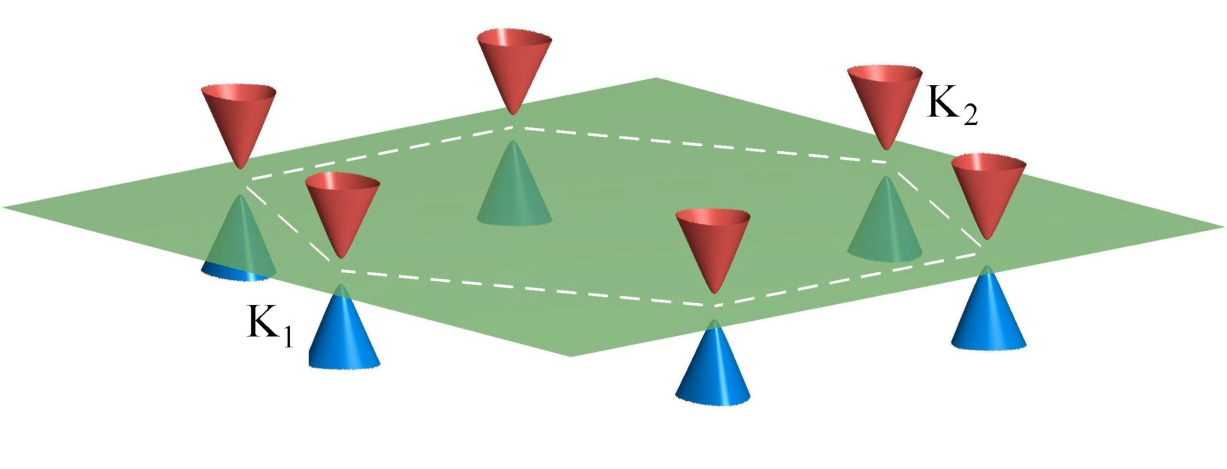
\includegraphics[width=0.7\linewidth]{Immagini/ValleyHall/band_graphene.pdf}
    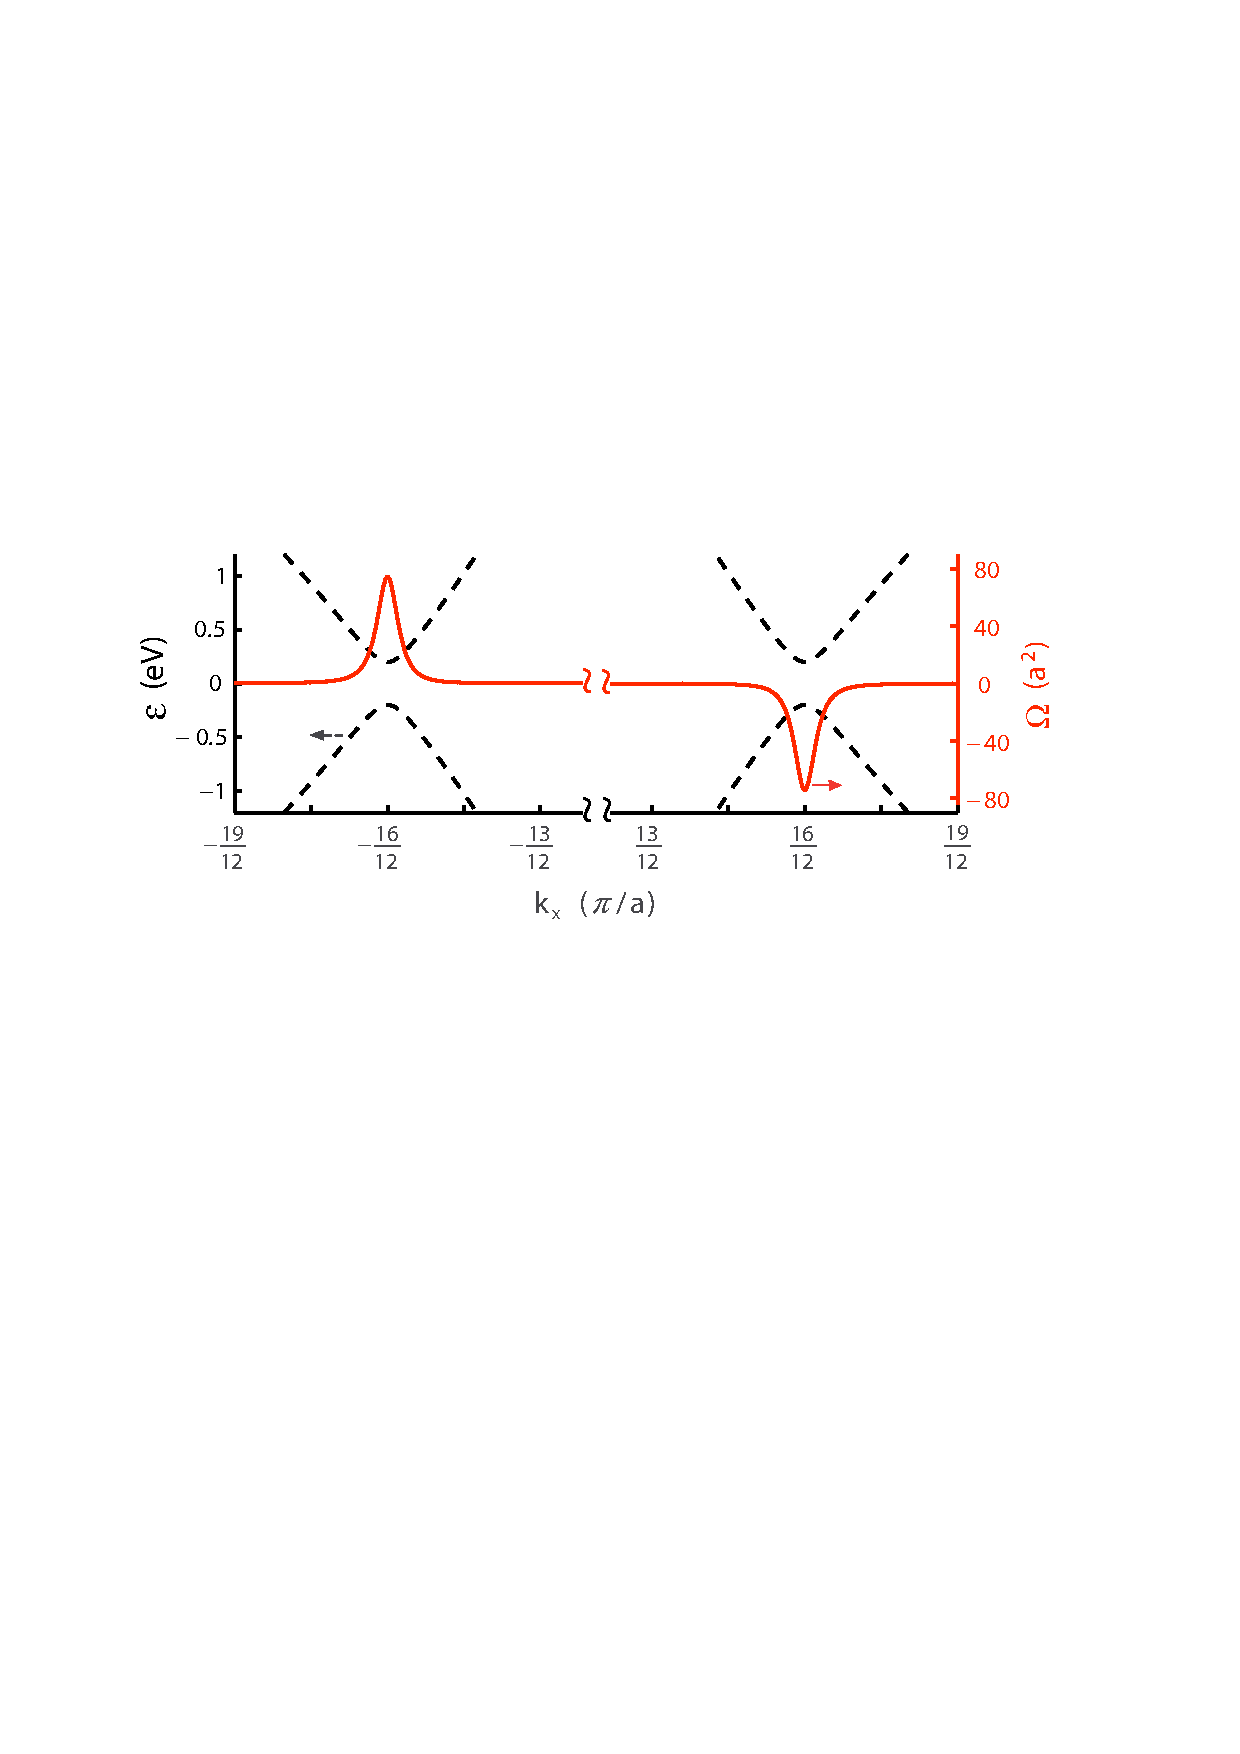
\includegraphics[width=0.7\linewidth]{Immagini/ValleyHall/curvature_graphene.pdf}
    \caption{In the top panel are displayed the Energy bands in 2D. In the bottom panel with the dotted line are displayed a section of the energy bands, and with the continuous red line the Berry curvature. Image taken from \cite{xiao2007valley}}
    \label{fig:cones}
\end{figure}
Notice how from figure \ref{fig:cones} most of the berry curvature lies near the cones. The nice thing about it is that to calculate the total curvature in any given band, we can calculate the Berry in the two cones, and then sum the results. This is because we know that the total Berry curvature over the band has to be quantized.

Now let's calculate the Chern number in any given cone from equation \ref{eq:dirac-curvature-q}.
\begin{equation}
    \begin{split}
        C=&\int \Omega_{q_xq_y}dq_xdq_y=\\
        =&\frac{\tau_z\Delta}2\int\frac{dq_xdq_y}{(q^2+\Delta^2)^{3/2}}=\\
        =&\frac{\tau_z\Delta}2\int\frac{2\pi q dq}{(q^2+\Delta^2)^{3/2}}=\\
        =&\pi\tau_z\Delta \frac 1{|\Delta|}\\
        =&\pi\tau_z\textrm{sign}(\Delta)\,.
    \end{split}
    \label{eq:dirac-curvature-total}
\end{equation}
This means that the two cones have opposite total Berry curvature, so the entire Brillouin zone has zero total Berry curvature. In the next section we are going to see how it is possible to give rise to a honeycomb system with a non zero total Berry curvature.


\section{The Haldane model}
    The Haldane model is a toy model of a spinless particle in a honeycomb lattice purposely made to exhibits a nonzero quantization of the Hall conductance a in the absence of an external magnetic field.\\
    The idea is to start with the classic nearest neighbor hopping with hopping parameter $t_1$, and then to break time reversal symmetry, Haldane introduced the next-nearest neighbour hopping parameter that is a imaginary number $t_2e^{i\phi}$ (figure \ref{fig:second-nearest}).
    \begin{figure}[h]
        \centering
        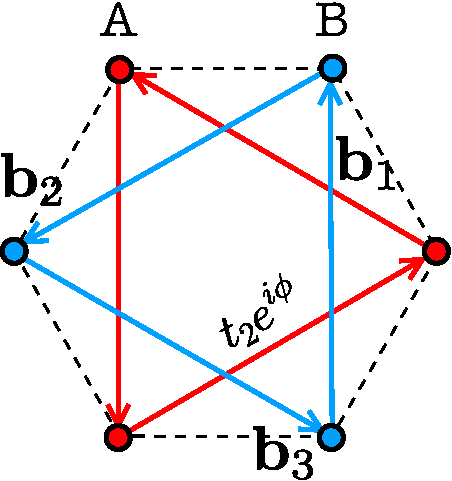
\includegraphics[width=0.5\textwidth]{Immagini/ValleyHall/Haldane-second-nearest.pdf}
        \caption{Honeycomb lattice showing nearest neighbor hopping with dashed line and next-nearest neighbor with the colored arrows, the red ones link only the atoms in the $A$ sites, while the blue one link the atoms in the $B$ sites. The transition amplitudes for the next-nearest are complex. Image adapted from \cite{topocondmat}.}
        \label{fig:second-nearest}
    \end{figure}
    The full Hamiltonian becomes 
    \begin{equation}
        H(\vect k)=H_0(\vect k) +\Delta\sigma_z -2t_2\sigma_z\tau_z\sin\phi\sum_i \sin(\vect k\cdot \vect b_i)\,.
    \end{equation}
    Where $\Delta$ is a mass term and $\vect b_i$ are the vectors that unite the atoms in the same sublattice site (figure \ref{fig:second-nearest}).
    Near the Dirac cones it assumes this form:
    \begin{equation}
            H(\vect k)=\hbar v_\textrm{F}(\sigma_x\tau_zk_x+\sigma_yk_y) +
            (\Delta - \tau_z\Delta_T\sin\phi)\sigma_z\,,
    \end{equation}
    Where
    \begin{equation}
        \Delta_T=2t_2\sum_i \sin(\vect K\cdot \vect b_i)\,.
    \end{equation}
    Notice ho the $\sigma_z$ term now has a $\tau_z$ term in it. Effectively this is the same as taking a massive Dirac Hamiltonian and then sending $\Delta\to\Delta + \tau_z\Delta_t\sin\phi$. This means that we can use equation \ref{eq:dirac-curvature-total} to calculate the Chern number.
    
    \begin{equation}
        C=\pi\tau_z\textrm{sign}(\Delta - \tau_z\Delta_T\sin\phi)\,.
    \end{equation}
    Notice how in this case, if $\Delta<|\Delta_T\sin\phi|$ the Chern number is $C=\pi$ and since it doesn't depend on the valley index both valleys have the same Chern number, and the total Berry curvature of the band is $2\pi$, making the material topological.\\
    If $\Delta = |\Delta_T\sin\phi|$ then we have that one of the two cones is closed, while if $\Delta>|\Delta_T\sin\phi|$ then both cones are open and the Chern number of the full band is 0, so the material is non-topological.\\
    To go to the topological state to the non-topological one the gap has to close in one of the two valleys (figure \ref{fig:gaps-topo-haldane}).
    \begin{figure}[h]
        \centering
        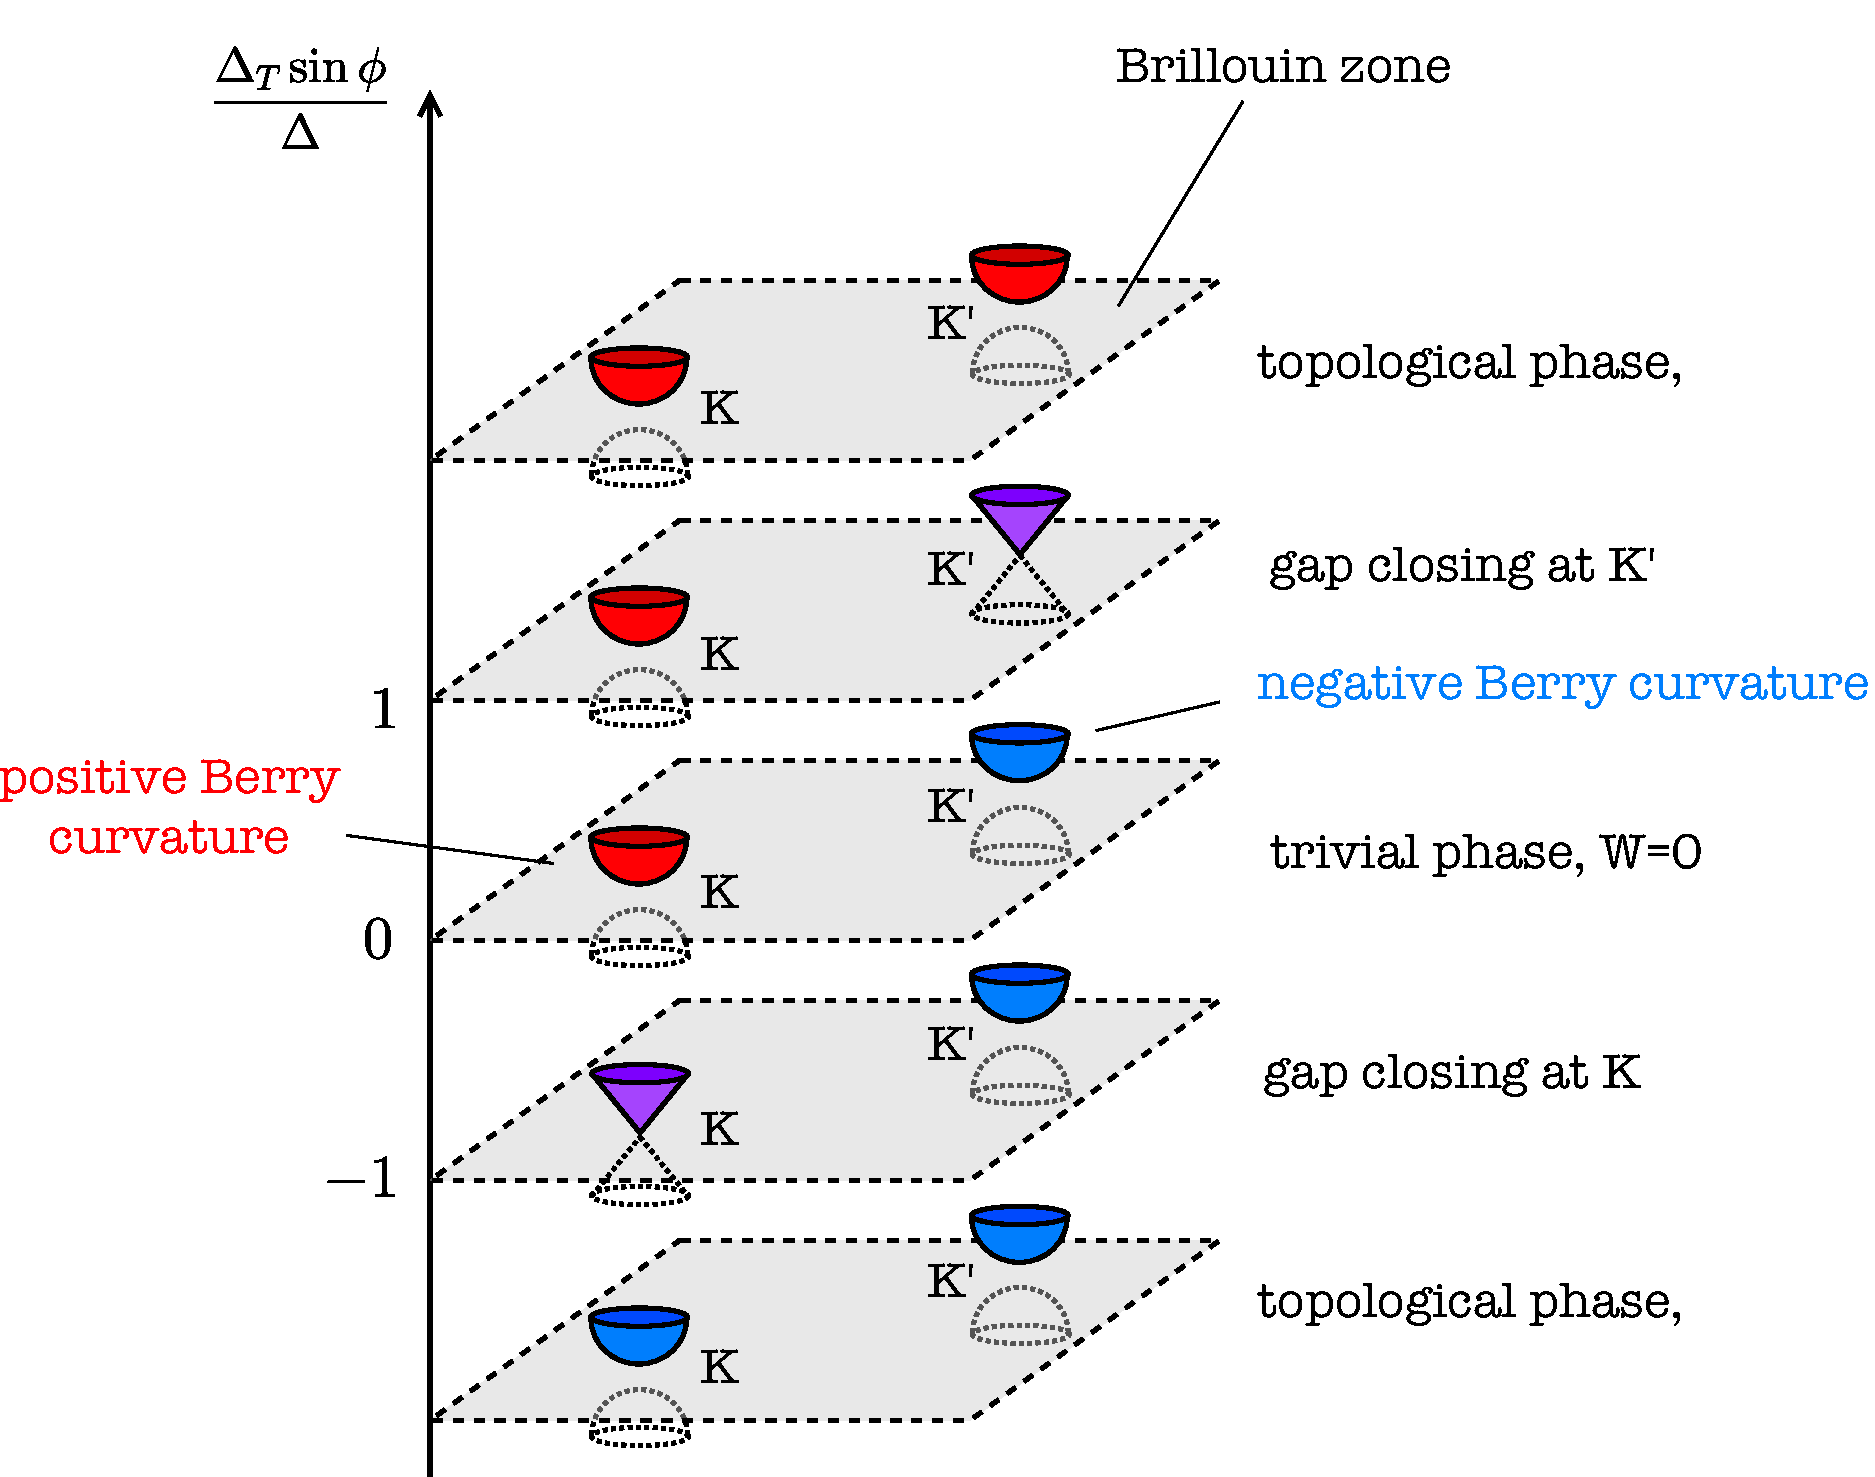
\includegraphics[width=\textwidth]{Immagini/ValleyHall/phasediagram-haldane.pdf}
        \caption{Phase diagram showing the topological phases ($\Delta<|\Delta_T\sin\phi|$), the trivial ones ($\Delta>|\Delta_T\sin\phi|$) and the phase change happens in the points where $\Delta = |\Delta_T\sin\phi|$. Image adapted from \cite{topocondmat}.}
        \label{fig:gaps-topo-haldane}
    \end{figure}\\
    Although this model seems unphisical it will be of crucial importance when explaining the Spin Hall effect.% so much so that this model, along with his other work made Haldane earned him the Nobel prize in Physics.